\section{Grueneisen relaxation photoacoustic microscopy (GR-PAM) theory}

In this section the Grueneisen effect is characterized theoretical and the application to microscopy is shown. Furthermore, the influence of varying laser wavelengths to GR-PAM is studied and a method to determine the absorption coefficient $\mu_a$ is presented. 

\subsection{The Grueneisen effect}
\label{sec:GReffect}
The initial pressure rise is defined by $p = \Gamma \mu_a F$ as discussed in chapter \ref{sec:photoeffect}. There the Grueneisen parameter $\Gamma$ is given by

\begin{equation}
\Gamma = \frac{\beta(T) \cdot c_s^2(T)}{C_p(T)}
\label{eq:gamma(T)}
\end{equation}

$\beta$ is the thermal expansion coefficient, $c_s$ is the speed of sound and $C_p$ is the specific heat capacity at constant pressure. All components of $\Gamma$ are temperature dependent. The change of the PA in terms of temperature is called Grueneisen effect. \\
The main contribution to this change comes from $\beta$. It rises at about 97~\% by a temperature change from 20~$^\circ$C to 40~$^\circ$C. There the contribution from $c_s$ and $C_p$ is less than 4~\% and 1~\% \cite{waterproperties, Tian:dualPulse}. 
This leads to the conclusion, that the Grueneisen parameter primarily depends on $\beta$. \\
Figure \ref{fig:GeffectPaper} shows the dependence of pressure amplitude from temperature. The measured amplitudes are normalized against the pressure amplitude at 26~$^\circ$C. 

\begin{figure}[H]
	\centering
	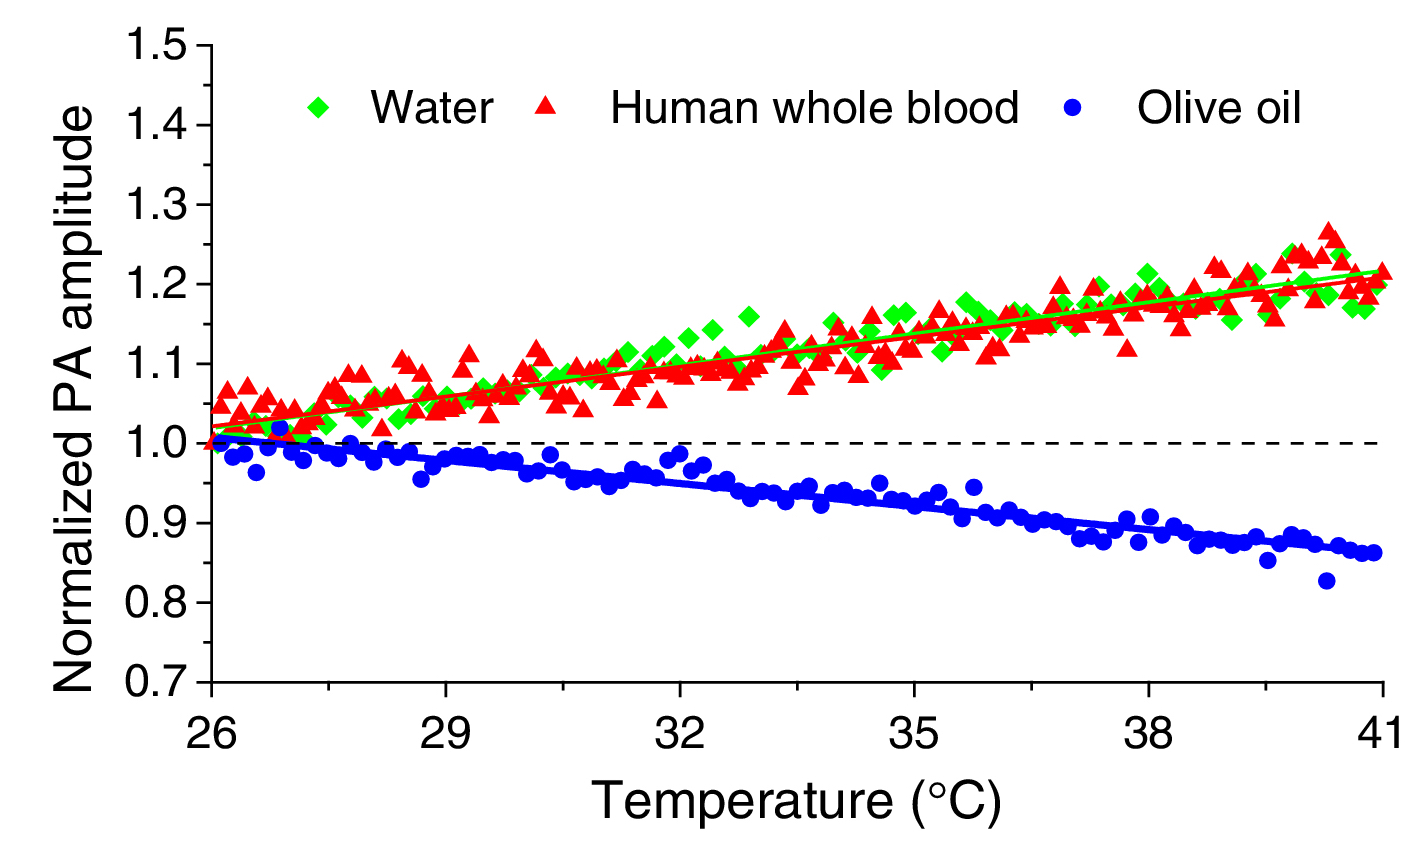
\includegraphics[width = 0.75\textwidth, height=0.3\textheight]{03_GR-PAM_theory/images/GeffectPaper.jpeg}
	\caption{Normalized pressure amplitude in dependence of temperature for water, human whole blood and olive oil. \cite{Tian:15}}
	\label{fig:GeffectPaper}
\end{figure}

It can be seen that the amplitude of water and blood rises while the one for olive oil decreases. Therefore the Grueneisen effect can be used to establish a contrast between thermal differing properties of the sample compounds. For example blood and fatty tissue can be separated \cite{Tian:15}. Another advantage is that most physical parameters of tissue have a strong temperature dependence \cite{Jacques:opticalPropsBiotissue}. 

\subsection{Dual pulse technique}
\label{sec:dualPulseTechnique}

In order to make the Grueneisen effect usable for microscopy, a significant temperature rise has to be employed into the area of interest. This can be done with a two laser pulse process sketched in figure \ref{fig:doublePulse}.\\
The laser pulses have to be in a nanosecond range. The first one at time $t_1$, called heating pulse, applies a significant temperature rise into the area of interest. The second one, called detecting pulse, is delivered to the sample with a submicrosecond delay and excites a second pressure wave, but this one is modified due to the Grueneisen effect. 

\begin{figure}[H]
	\centering
	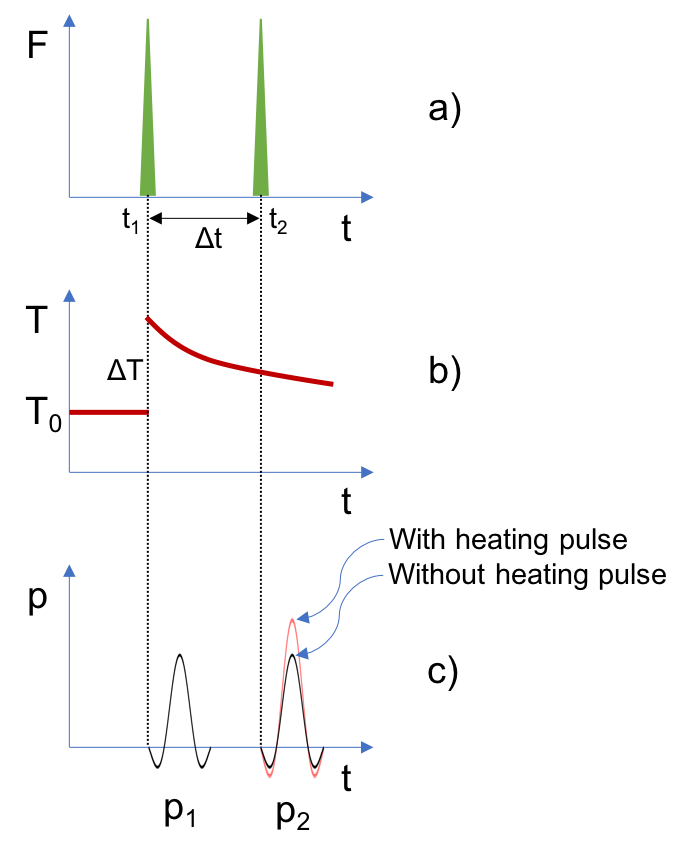
\includegraphics[width = 0.5\textwidth]{03_GR-PAM_theory/images/dualPulse.png}
	\caption{Signal generation sequence for GR-PAM with G $>0$.}
	\label{fig:doublePulse}
\end{figure}

The initial pressure rise p$_1$ is identical to equation \ref{eq:p_0}, with equilibrium temperature $T_0$ and $\Gamma_0$. For the following considerations a heat conversion coefficient $\eta_{th}$ were added, this coefficient pools all side effects and acts as a correction factor

\begin{equation}
	p_1 = \Gamma \eta_{th} \mu_a F
\end{equation}
\\
If the second laser pulse hit the sample before the temperature has reached the equilibrium state again, a pressure rise p$_2$ is formed given by

\begin{equation}
	p_2 = \Gamma(T_0 + \Delta T, \Delta t) \eta_{th} \mu_a F_2
	\label{eq:grPA2}
\end{equation} 

\begin{equation}
\Gamma(T_0 + \Delta T, \Delta t) = \Gamma_0 + G \cdot \Delta T \cdot \tau(\Delta t)
\end{equation} 
\begin{equation}
\Delta T = \eta_{th} \mu_a F_1
\end{equation} 
\\
there G is a coefficient that relates to the change of the Grueneisen parameter and $\tau$ a relaxation function (compare Figure \ref{fig:doublePulse} b) \cite{Ma:GRPAMinVivo,Tian:15}. As seen in Figure \ref{fig:GeffectPaper} the change of the Grueneisen parameter can either be positive or negative and thus G can be. Therefore G in Figure \ref{fig:doublePulse} is positive, this results in a higher amplitude p$_2$ than without heating. In order to make the difference visible, p$_1$ gets subtracted from p$_2$. 

\begin{equation}
	\Delta p = p_2 - p_1 = G \eta_{th}^2 \mu_a^2 F^2
	\label{deltaP}
\end{equation}
\\
This equation is only valid if F$_1$ = F$_2$. Otherwise additional terms emerge. It can be seen, $\Delta$p and therefore G depend quadratically on the fluence. This makes the Grueneisen effect a non-linear effect.\\

\subsubsection{Influence of laser-wavelength differences to GR-PAM}

In Figure \ref{fig:doublePulse} has to be considered that both pulses have the same wavelength. But systems can vary from this ideal configuration. Differing heating volumes for heating (V$_1$, $\lambda_1$) and detecting (V$_2$, $\lambda_2$) pulse are a consequence. Furthermore, a different absorption coefficient can be valid. Therefore three cases can be deduced\\

\begin{itemize}
\centering
\item[1) ] $\lambda_1 = \lambda_2 ;\, \mu_a(\lambda_1) = \mu_a(\lambda_2) ;\, \delta_1 = \delta_2 \, and\, V_1 = V_2$
\item[2) ] $\lambda_1 \neq \lambda_2 ;\, \mu_a(\lambda_1) < \mu_a(\lambda_2) ;\, \delta_1 > \delta_2 \, and\, V_1 \supset V_2$
\item[3) ] $\lambda_1 \neq \lambda_2 ;\, \mu_a(\lambda_1) > \mu_a(\lambda_2) ;\, \delta_1 < \delta_2 \, and\, V_1 \subset V_2$
\end{itemize}

Case 1) is the ideal case. Both pulses have the same wavelength and thus the same $\mu_a$. Therefore penetration depth equals heating volume. In 2) the detection volume is embedded into the heating volume. Here the non-linear effect is higher than in case 1). Case 3) is vice versa, the detection volume is bigger and therefore the effect smaller \cite{Tian:dualPulse}.

\subsubsection{Measurement  of the absorption coefficient $\mu_a$}

In order to get to know the absorption coefficient of liquids the setup shown in figure \ref{fig:mu_aSetup} were built. \\
A pulsed laser were coupled into a optical fiber to deliver the light to the setup. The laser-wavelength have to be tunable, to perform the measurement over the desired wavelength range.  

\begin{figure}[H]
	\centering
	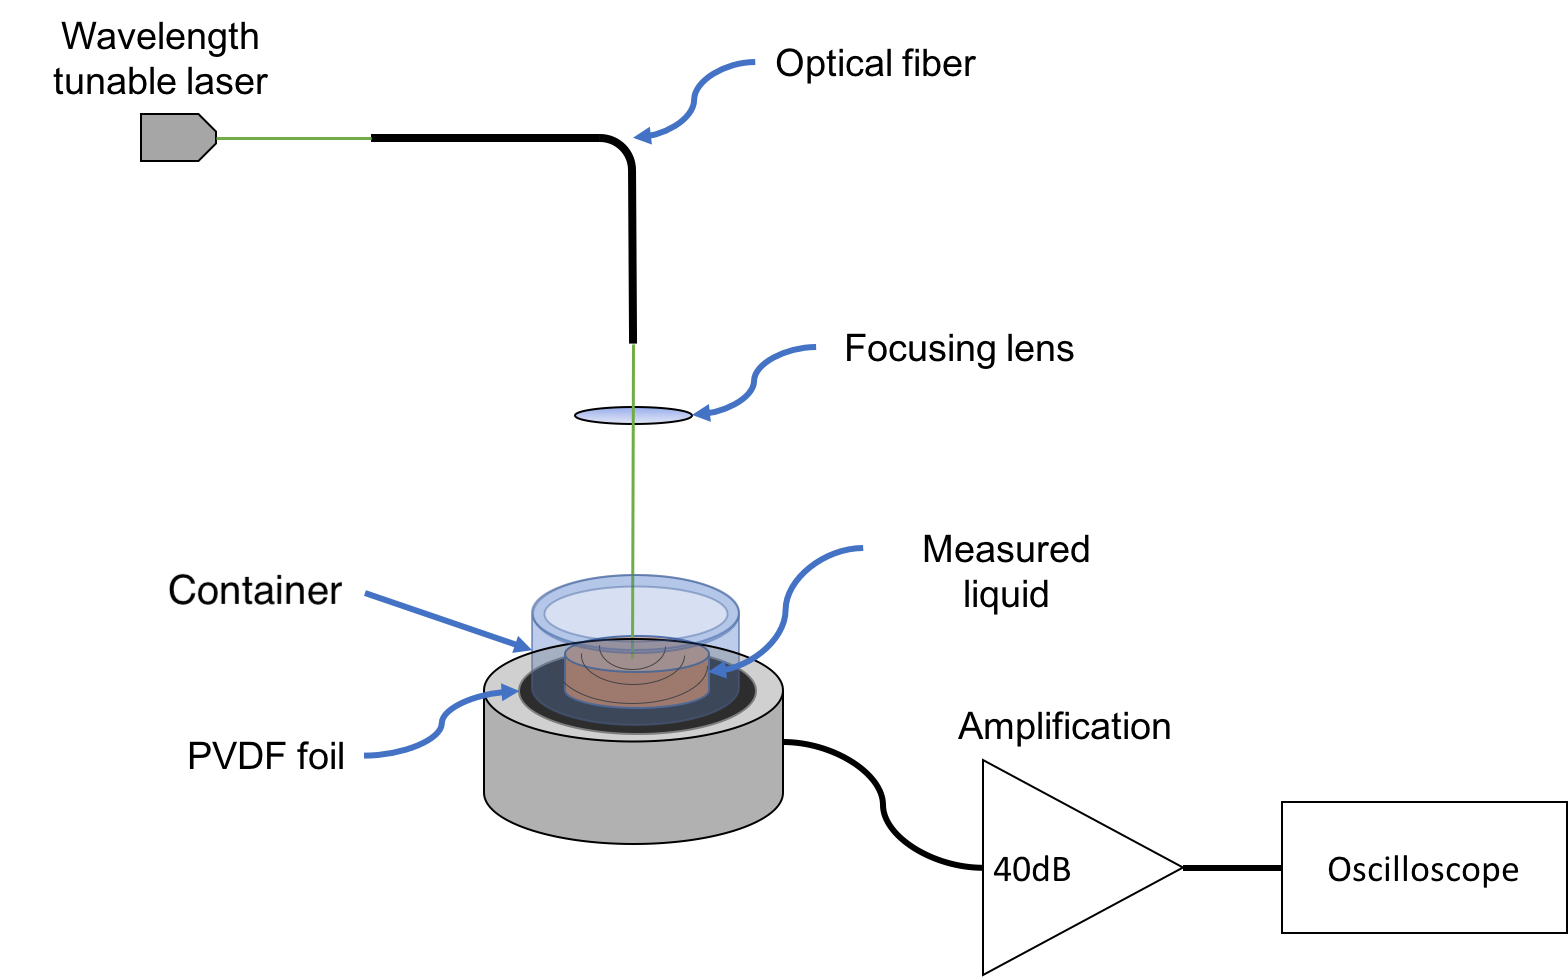
\includegraphics[width = \textwidth]{03_GR-PAM_theory/images/mu_aSetup.jpg}
	\caption{Measuring setup to determine the absorption coefficient.}
	\label{fig:mu_aSetup}
\end{figure}

In order to illuminate a certain area of the absorbing liquid, a bi-convex lens were used. The typical used liquid height is 5~$mm$. However, it has to be considered that liquids which have a high acoustic damping should have a lower level in order to get a decent signal. The container were sealed at the bottom with a thin polymer membrane to couple the soundwave with a minimum loss to the PVDF foil, which were placed on top of a metal housing. PVDF is a polymer with piezo-electric properties and therefore capable to detect ultrasonic waves. The foil generates a voltage signal, which is amplified by 40~$dB$ and displayed on an oscilloscope. The pressure rise can be written as 

\begin{equation}
p(t) = p_0 \cdot exp(-\mu_a(\delta-c_s t))
\end{equation}  
\\
where $p_0$ is the initial pressure rise (formula \ref{eq:p_0}) and $\delta$ the penetration depth (which is neglected for the fit) \cite{demtroder:ExPhysik}. 

\begin{figure}[H]
	a)
	\begin{minipage}{0.5\textwidth}		
		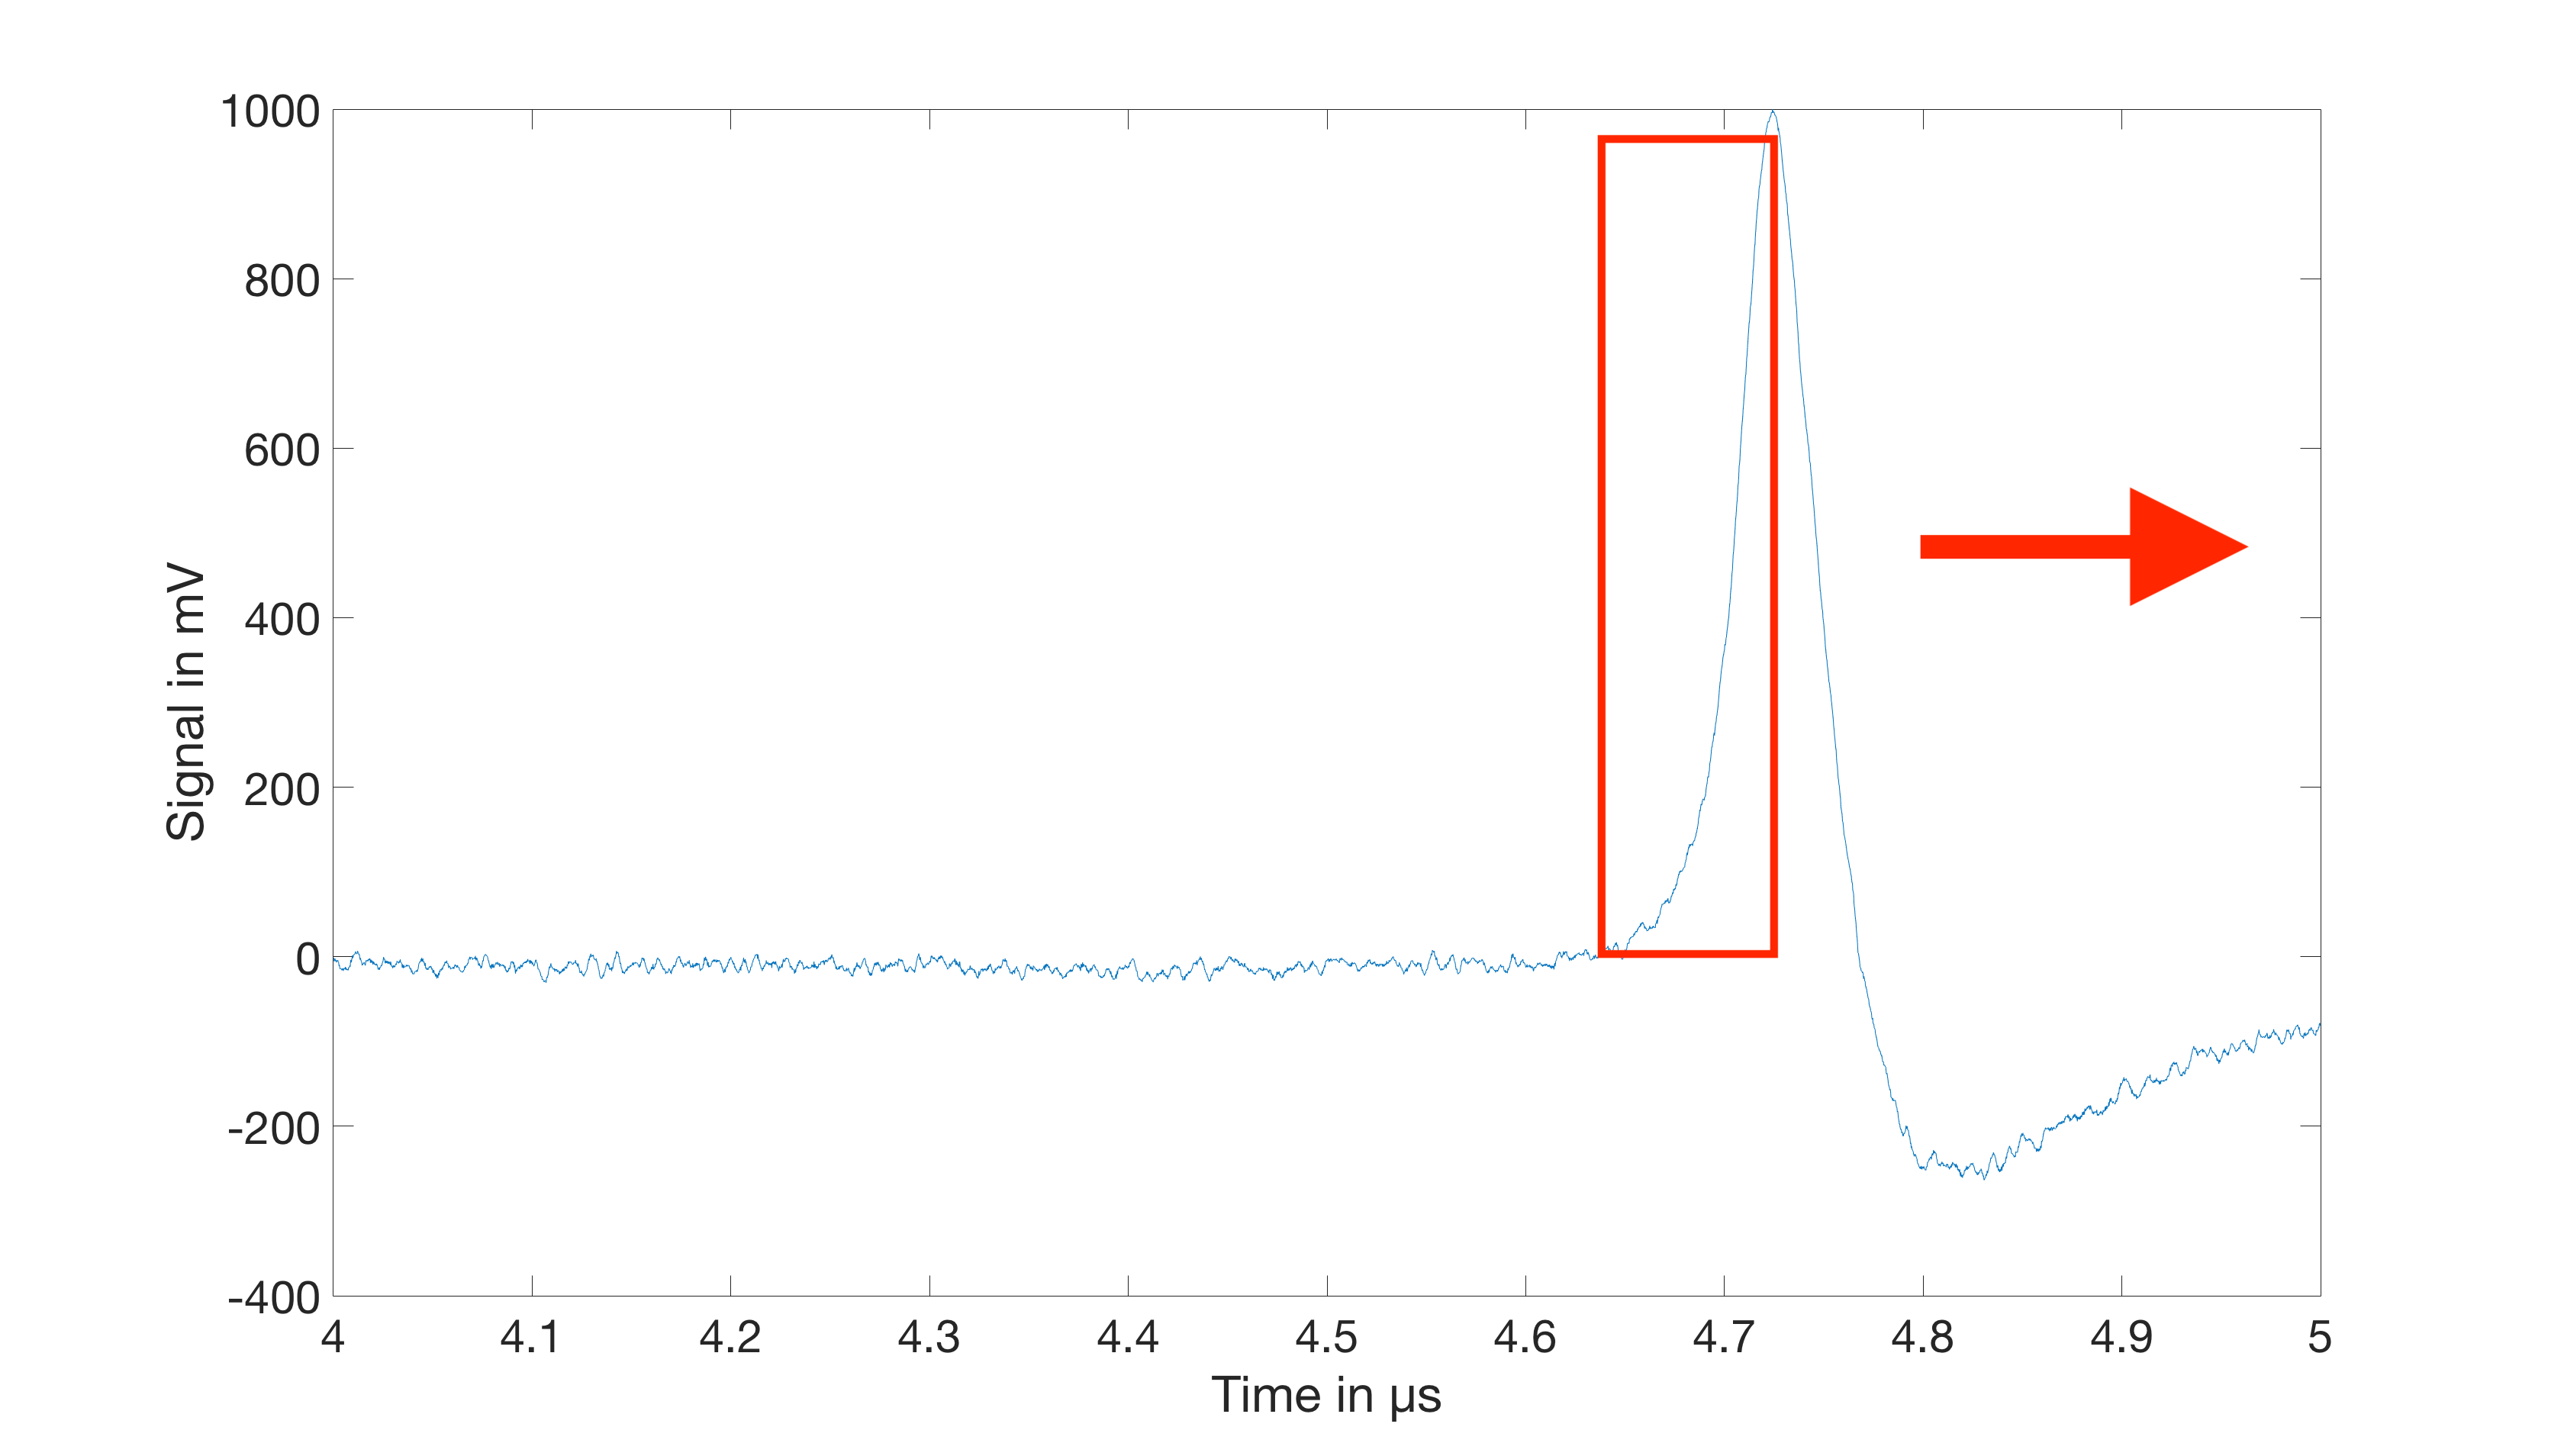
\includegraphics[width = \textwidth, height=0.25\textheight]{03_GR-PAM_theory/images/mu_aSig.png}
	\end{minipage}
	b)
	\begin{minipage}{0.5\textwidth}		
		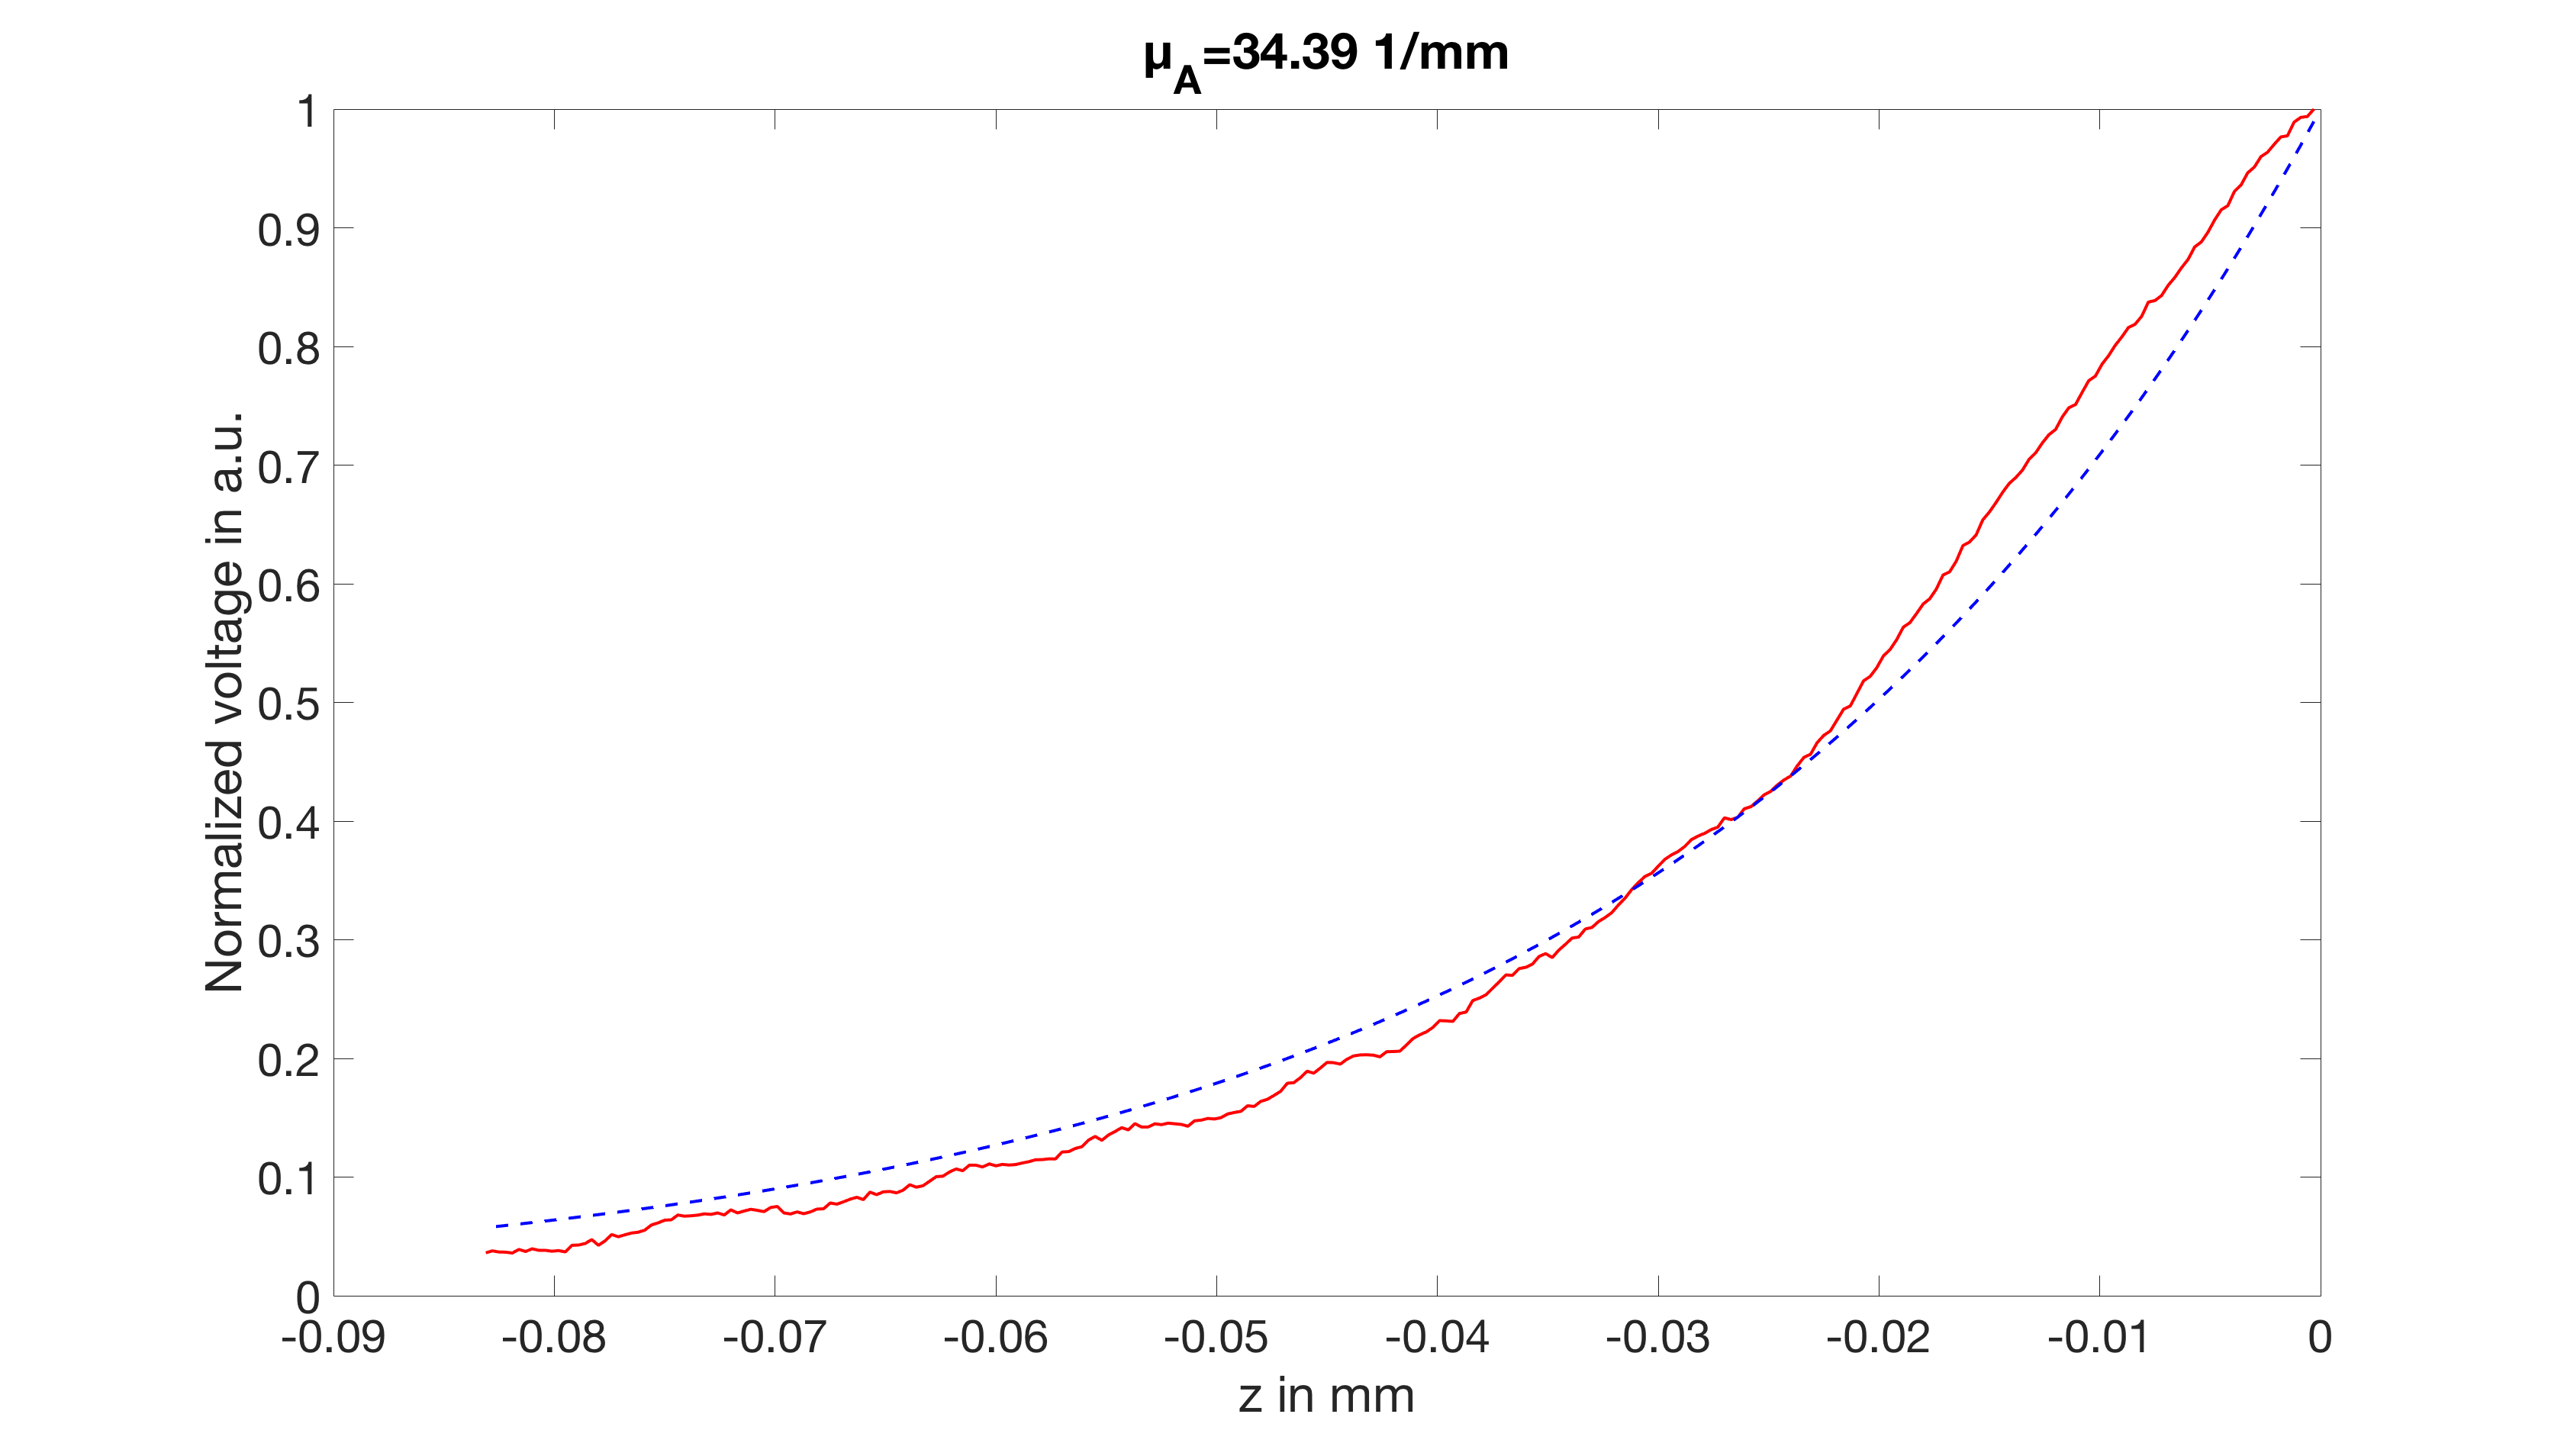
\includegraphics[width = \textwidth, height=0.25\textheight]{03_GR-PAM_theory/images/mu_aFit.png}
	\end{minipage}	
	\caption{In a) a typical PA signal is shown, there the rising part is taken to fit in an exponential function shown in b). The x-axis in b) is converted from a time scale into a depth scale, there zero marks the maximum penetration depth taken. In b) the red line marks the measured data and the dashed blue line is the fit function.}
	\label{fig:mu_aSigFit}
\end{figure}

In figure \ref{fig:mu_aSigFit} the procedure to determine $\mu_a$ is shown. At first a laser pulse were shot onto the liquid and the generated PA signal were recorded. Afterwards the data were loaded into a Matlab program to select the rising edge of the PA signal. A fit function then determines the most suitable $\mu_a$, which is displayed in a plot. 

\subsection{Resolution considerations}
\label{sec:resConGR}

In order to determine the possible theoretical resolution that can be achieved, a 2D Gaussian distribution, for the fluence in lateral direction, can be supposed. The PA$_1$ that is generated by the first laser pulse can be derived by the spatial integration of p$_1$. 

\begin{equation}
	\mathrm{PA}_1 = k_{loss} \Gamma_0 \eta_{th} Q \iint\mu_a(x,y) \frac{1}{\pi w^2} \exp{\left(-\frac{x^2+y^2}{w^2}\right)} \mathrm{d}x\mathrm{d}y
	\label{eq:PA1}
\end{equation}
\\
There the PA is the measured voltage signal. The transformation of a pressure wave into a voltage signal, the detection sensitivity and the appearing losses are considered by a constant $k_{loss}$. For the assumption, that the integration can be performed independently from the z-direction, can be followed, that there are only contributions to k. Further $Q$ is the pulse energy and $w_0$ is the waist of the Gaussian beam shown in Figure \ref{fig:focusWaist} \cite{Bessel:GRPAM, Wang:GRPAM}. 

\begin{figure}[H]
	\centering
	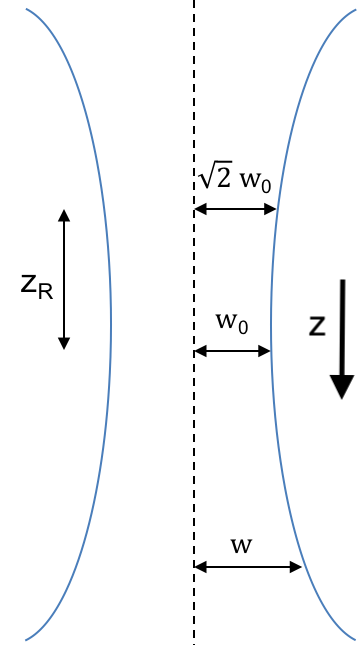
\includegraphics[width = 0.25\textwidth, height=0.3\textheight]{03_GR-PAM_theory/images/focusWaist.png}
	\caption{Optical focus waist, where $w_0$ is the smallest waist radius, $z_R$ the Rayleigh length (distance from $w_0$ there the waist radius is $\sqrt{2}$ $w_0$) and $w$ the distance from the optical axis.}
	\label{fig:focusWaist}
\end{figure}

Analogue to PA$_1$, PA$_2$ is determined by

\begin{multline}
	\mathrm{PA}_2 = \underbrace{k_{loss} \Gamma_0 \eta_{th} Q \iint \mu_a(x,y) \frac{1}{\pi w^2} \exp{\left(-\frac{x^2+y^2}{w^2}\right)} \mathrm{d}x \mathrm{d}y}_{\mathrm{I}} \; + \\ \underbrace{k_{loss} G \eta_{th}^2 Q^2 \iint \mu_a(x,y)^2 \frac{1}{\pi^2 w^4} \exp{\left(-\frac{x^2+y^2}{\frac{1}{2}w^2}\right)} \mathrm{d}x\mathrm{d}y}_{\mathrm{II}}
	\label{eq:PA2}
\end{multline}
\\
Equation \ref{eq:PA2} consists of two parts. Part $I$ is the same as PA$_1$ (\ref{eq:PA1}). But part $II$ is induced by the Grueneisen effect, resulting of the first laser pulse preheating and the excitation of the second laser pulse. The assumption that F$_1$~= ~F$_2$ is still valid. If the generated PA$_1$ is subtracted from PA$_2$, $\Delta \mathrm{PA}$ is given by

\begin{equation}
\begin{split}
	\Delta \mathrm{PA} &= \mathrm{PA}_2 - \mathrm{PA}_1\\
	&= k_{loss} G \eta_{th}^2 Q^2 \iint \mu_a^2(x,y) \frac{1}{\pi^2w^4} \exp{\left(-\frac{x^2+y^2}{w^2/2}\right)} \mathrm{d}x\mathrm{d}y
	\end{split}
\end{equation}
\\
In order to determine the lateral resolution of GR-PAM a point target can be scanned in the x - y plane. Consequently the point spread function is given by 

\begin{equation}
\Delta \mathrm{PA} (x,y) = k_{loss} G \eta_{th}^2 Q^2 \mu_a^2 \frac{1}{\pi^2w^4} \exp{\left(-\frac{x^2+y^2}{w^2/2}\right)} 
\end{equation}
\\
which correspond to a 2D Gaussian distribution with a waist $\sigma$ of $w/\sqrt{2}$. In comparison, OR-PAM gives the following distribution. 

\begin{equation}
\mathrm{PA_{OR-PAM}} (x,y) = k_{loss} \Gamma_0 \eta_{th} Q \mu_a \frac{1}{\pi w^2} \exp{\left(-\frac{x^2+y^2}{w^2}\right)} 
\end{equation}
\\
This follows a $\sigma$ of $w$ and therefore a higher lateral resolution of GR-PAM compared to OR-PAM by the factor $\sqrt{2}$ \cite{PhysRevLett.113.174301}.\\
The axial resolution of GR-PAM can be determined by analyzing the Gaussian beam profile depending on the z-direction, shown in figure \ref{fig:focusWaist}.
There the waist width $w$ is defined by

\begin{equation}
w(z)^2 =  w_0^2 \left(1 + \frac{z^2}{z_R^2}\right)
\end{equation}
\\
The GR-PAM signal for a planar target with uniformly distributed $\mu_a$ is 

\begin{equation}
\Delta \mathrm{PA} = k_{loss} G \eta_{th}^2 Q^2 \mu_a^2 \frac{1}{2 \pi^2w^2} 
\end{equation}
\\
There the OR-PAM signal for the same target is

\begin{equation}
\mathrm{PA_{OR-PAM}} = k_{loss} \Gamma_0 \eta_{th} Q \mu_a 
\label{eq:PA_OR_PAM}
\end{equation}
\\
This follows for $z = \pm z_R$, that the GR-PAM amplitude reduces by half, when the laser beam is focused onto the absorbing plane. Therefore the axial FWHM is $2\cdot z_R$, following optical axial sectioning capabilities for GR-PAM. It is evident that OR-PAM has no optical axial sectioning for planar targets as described by formula \ref{eq:PA_OR_PAM}. Due to no dependence on the focal distance \cite{PhysRevLett.113.174301}.\\
In table \ref{tab:resCompare} the comparison of the possible resolution power for OR-PAM and GR-PAM is collected.

\begin{table}[H]
	\centering
	\caption{Comparison of the theoretical possible resolutions that can be achieved with OR-PAM and GR-PAM \cite{Wang:GRPAM}.}
	\begin{tabular}{| m{1.7cm} | c | c |}
		\hline
		&OR-PAM&GR-PAM \\ \hline
		\centering Axial \newline resolution&no optical resolution&$2\cdot z_R$ \\ \hline
		\centering Lateral \newline resolution&$2 \cdot w_0$&$\sqrt{2} \cdot w_0$\\	\hline
	\end{tabular}	 
	\label{tab:resCompare}
\end{table}



